\sectionlink{Nambu-GoldstoneモードのEFT}


対称性は、あらゆるEFTを定める基本要素の一つであると論じてきた。すなわち、不変な項はすべて有効作用に含めるべきである。実際には、問題となる対称性のもとで線形に変換する場、つまり、ある定数行列$M$に対して$\varphi^i \to M^i{}_j \varphi^j$という形の変換則に従う場を扱う場合、これはかなり容易に実現できる。\footnote{もちろん、いくらでも複雑な場の再定義を行うことによって、変換則を好きなだけ複雑にすることは常に可能である。Steven Weinbergの「理論物理学の進歩の第三法則」は、この可能性について述べている。{\it 「物理系を記述するために、どのような自由度を使ってもよい。しかし、間違った自由度を使えば、後悔することになる」}~\cite{Weinberg:1981qq}。}この場合、不変となるように添字を縮約すればよい。しかし、自発的に破れた対称性は、それによって生じるGoldstoneモード上では非線形に実現される。この場合、可能な不変演算子をすべて書き下すことは、必ずしも容易ではない。本章の前半では、最も軽いQCD束縛状態を記述するEFTであるカイラル摂動論（CPT）を通して、非線形に実現される対称性を導入する。このEFTには、前章で議論したものに加えて、さらにいくつかの微妙な点が現れる。本章の後半では、非線形に実現される対称性のもとで不変な有効作用を書き下すための一般的な手法である、剰余空間構成を導入する。その過程で、近似的な対称性やアノマリーをもつ対称性を備えたEFTの扱い方も学ぶ。



\subsectionlink{カイラル摂動論} \label{sec: CPT}



陽子や中性子よりも軽いQCD束縛状態を調べたいとしよう。この場合、質量がGeVスケール以上のすべてのSM粒子を積分消去して、得られる有効理論を用いればよい。残るクォーク、すなわち$u$、$d$、$s$は、低エネルギーでは次の有効作用によって記述される。
%
\begin{align} \label{SM action below 1 GeV}
	S = \int d^4 x \left\{ \sum_{j=u,d,s} \bar \Psi_j (i \gamma^\mu D_\mu - m_j ) \Psi_j - \frac{1}{4} F_{\mu\nu} F^{\mu\nu} - \frac{1}{2} \mbox{Tr} \, G_{\mu\nu} G^{\mu\nu} + \, \dots \right\} , 
\end{align}
%
ここで、$D_\mu \Psi_j = (\partial_\mu - i q_j A_\mu - i g \, G_\mu ) \Psi_j$であり、$A_\mu$と$G_\mu$は光子場とグルーオン場、$F_{\mu\nu}$と$G_{\mu\nu}$はそれぞれの場の強さである。カラー添字は以下の議論では役割を果たさないため、一貫して省略する。上のLagrangianの省略記号は、GeVより低いエネルギーで抑制される、あらゆる種類の「繰り込み不可能」な項を表す。とりわけ、クォークと軽いレプトンの間の相互作用もこれに含まれる。

残る三つのクォークの質量はいずれも、この問題における唯一の他のスケール、すなわち閉じ込めに関係するQCDスケール$\Lambda_{\rm QCD}  \simeq 300$ MeVより小さい。したがって、まずクォーク質量を無視して束縛状態を調べることは、妥当な近似と思われる。確かに、この近似は、質量が$\mathcal{O}(1)$ MeVの$u$、$d$クォークに対しては、$m_s \simeq 100$ MeVである$s$クォークに対してよりもよく成り立つ。それでも、この注意点を念頭に置きつつ議論を進め、さらに電磁結合も無視することにしよう。有限の質量と電磁相互作用の効果は、次節で再び導入する。この極限では、クォーク場を次のように定義される左巻き成分と右巻き成分に分けると便利である。
%
\begin{align}
	\Psi^j_L = \tfrac{1}{2} (1 - \gamma^5) \Psi^j, \qquad \qquad \quad \Psi^j_R = \tfrac{1}{2} (1 + \gamma^5) \Psi^j, 
\end{align}
%
すると、上の作用は次のようになる。
%
\begin{align} \label{approximate SM action below 1 GeV}
	S \simeq \!\int d^4x \!\!\! \sum_{j=u,d,s} \!\! \left[ \bar \Psi_L^j i \gamma^\mu (\partial_\mu - i g \, G_\mu ) \Psi_L^j + \bar \Psi_R^j i \gamma^\mu (\partial_\mu - i g \, G_\mu ) \Psi_R^j \right] - \frac{1}{2} \mbox{Tr} \, G_{\mu\nu} G^{\mu\nu} + \, \dots .
\end{align}
%

この作用は、いくつかの大域的対称性のもとで不変である。まず、共形変換のもとで不変である。これは、式\eqref{approximate SM action below 1 GeV}に質量スケールが存在しないことから従う。それにもかかわらず、量子効果によってQCD結合がエネルギーとともに走り、スケール$\Lambda_{QCD}$で相互作用が強くなるため、特定の質量スケールが動的に生成される。言い換えると、共形不変性にはアノマリーがある。量子効果によって破られるため、完全な理論の対称性ではないのである。

作用\eqref{approximate SM action below 1 GeV}は、左巻きクォークと右巻きクォークに対する独立な$U(3)$変換のもとでも不変である。
%
\begin{align}
	(\Psi_L^i)' = L^i{}_j \Psi_L^j, \qquad \qquad \quad (\Psi_R^i)' = R^i{}_j \Psi_R^j \ .
\end{align}
%
この対称性の群$U(3)_L \times U(3)_R$を、積$SU(3)_L \times SU(3)_R \times U(1)_V \times U(1)_A$に分解すると便利である。ここで$U(1)_V$は、すべてのクォーク場の位相を大域的に変更する変換に対応する。一方、$U(1)_A$は、左巻きクォークと右巻きクォークを互いに逆の位相で変換する。すなわち、
%
\begin{align}
	\Psi_L' = e^{i \alpha} \Psi_L, \qquad \qquad \quad \Psi_R' = e^{-i \alpha} \Psi_R \ .
\end{align}
%
これらの部分群は、それぞれ異なる立場にある。\high{軸性対称性}$U(1)_A$にはアノマリーがあり、したがって量子論の真の対称性ではない。この点については\ref{sec: chiral anomalies}節で詳しく述べる。さらに、強い相互作用によって、演算子$\bar \Psi^i_R \Psi_L^j$は次の形の非自明な真空期待値（vev）をもつ。
%
\begin{align} \label{chiral symmetry breaking}
	\langle \bar \Psi^i_R \Psi_L^j \rangle = v^3 \delta^{ij} ,
\end{align}
%
ここで$v \sim \Lambda_{\rm QCD}$である。この真空期待値は、\high{カイラル対称性}$SU(3)_L \times SU(3)_R$を、左巻きフェルミオンと右巻きフェルミオンが歩調をそろえて変換する対角部分群$SU(3)_V$へと自発的に破る。\footnote{アノマリーに基づく非常に一般的な議論によって、$SU(3)_L \times SU(3)_R$は、具体的には特定されない何らかの部分群へ自発的に破れなければならないことが示される~\cite{tHooft:1979bh}。}（$U(1)_A$対称性と共形対称性がそもそも真の対称性でないという事情がなければ、この真空期待値はそれらも自発的に破るはずである。）その結果、Goldstoneの定理により、この理論のスペクトルは（少なくとも）八つの質量ゼロの束縛状態、すなわち破れた対称性の生成子一つにつき一つのNambu-Goldstone（NG）モードを含まなければならない。最後に、式\eqref{chiral symmetry breaking}の真空期待値は、\high{バリオン対称性}$U(1)_V$を保つ。\footnote{正確には、弱い相互作用を考慮すると、バリオン対称性にもアノマリーがある。厳密に保存されるのは、バリオン数とレプトン数の差だけである。しかし、レプトン対称性はクォークとグルーオンに自明に作用するため、作用\eqref{SM action below 1 GeV}はバリオン対称性だけのもとでも不変に見える。これは、強い相互作用によってバリオン数が保存されることを意味する。}これは、クォークとグルーオンの束縛状態が、$U(1)_V$のもとで定まった電荷をもたなければならないことを意味する。

以下では、カイラル対称性の自発的破れに伴うNGモードのEFTを導く。このEFTは\high{カイラル摂動論}と呼ばれ、その展開パラメータは再び$E /\Lambda$という形の比になる。ここで$\Lambda$は、これから決定する何らかのUVスケールである。前章で扱ったトイモデルと比べると、このEFTには二つの新しい特徴がある。第一に、すでに指摘したように、作用\eqref{approximate SM action below 1 GeV}には質量スケールがまったく含まれない。そのため、強結合スケール$\Lambda$が何であるべきかは、すぐには明らかでない。特に、これは対称性の破れのスケール$v$と一致する必要はないことに注意してほしい。ただし、実際にはそれほどかけ離れた値にはならない。第二に、NG場はUV作用\eqref{approximate SM action below 1 GeV}に直接現れない。したがって、前章で行ったように、いくつかの重い場を単純に積分消去することでEFTを導くことはできない。強い相互作用のため、明示的なマッチング計算ができないのである。したがって、粒子の内容と対称性だけを指針とし、EFTの係数を実験によって決定すべき自由パラメータとして扱う必要がある。

対称性がNG場にどのように作用するかを調べるには、NG励起を、真空期待値に対する破れた変換が時空間で「緩やかに」変調されたものと考えると便利である。一定の破れた変換は、定義により、真空期待値\eqref{chiral symmetry breaking}を、それとは異なるが物理的には等価な真空期待値に変える。一方、NG励起は、時空の各点で真空を滑らかに変化させる。これはしばしば、NGモードが異なる真空を補間する、と表現される。この考えに基づき、$L(x) = R^\dag (x) = e^{i \pi^a(x) Q_a}$を満たす局所的な$SU(3)_L \times SU(3)_R$変換を、真空期待値\eqref{chiral symmetry breaking}に作用させる。ここで$\pi^a(x)$は八つのNG場であり、$Q_a$は$SU(3)$の生成子である。結果は次のようになる。
%
\begin{align}
	\langle \bar \Psi^i_R \Psi_L^j \rangle \to v^3 U^{ji} , \qquad \quad \text{ただし} \qquad \quad U (x) = L(x) \cdot R^\dag (x) = e^{2 i \pi^a(x) Q_a} .
\end{align}
%
したがって、NG励起は、$3 \times 3$複素行列$\langle \bar \Psi^i_R \Psi_L^j \rangle$の局所的な変形のうち、$SU(3)$変換$U(x)$で記述できる特定の変形に対応する。この変換は、行列の全体的な「大きさ」、すなわち行列式を保つことに注意してほしい。さて、一般の$SU(3)_L \times SU(3)_R$変換では$L(x) \to \tilde L \cdot L(x)$および$R(x) \to \tilde R \cdot R(x)$となるので、
%
\begin{align} \label{chiral transformations U}
	U \to U' = \tilde L \cdot  U \cdot \tilde R^\dag .
\end{align}
%
同様に、$SU(3)_L \times SU(3)_R$の生成子は$U(1)_V$の生成子と可換であるため、$\pi^a$のバリオン電荷がゼロでなければならないことも、容易にわかる。

式\eqref{chiral transformations U}の形のカイラル変換は線形であるため、そのもとで不変な$U$の有効作用を書き下すことは難しくない。$U$はユニタリなので、$U^\dag U$という形の積はどれも自明に不変になる。このため、$U$と$U^\dag$の両方に加えて、微分を用いる必要がある。少し考えれば、二つの微分を用いて書ける不変な項は一つしかないことがわかる。したがって、NGボソンの有効作用は次の形になる。
%
\begin{align} \label{CPT action}
	S = \int d^4 x \left\{ - \frac{f^2}{4} \mbox{Tr} \, ( \partial_\mu U^\dag \partial^\mu U ) + \dots \right\} ,
\end{align}
%
ここで$1/4$という因子は後の便宜のために導入しており、省略記号は微分を二つより多く含むすべての項を表す。このEFTには、多くの注目すべき特徴がある。
%
\begin{itemize}
	\item 有効作用は、NG場のべきで展開すると無限個の項を含むにもかかわらず、微分展開の最低次では単一のパラメータ$f$にしか依存しない。四次まで書くと、
%
\begin{align} \label{CPT expanded action}
	S = \int d^4 x \, f^2 \left\{ - \frac{1}{2} \partial_\mu \pi_a \partial^\mu \pi^a + \frac{1}{6} f_{abc} f_{de}{}^c \pi^b \pi^e \partial_\mu \pi^a \partial^\mu \pi^d  + \dots \right\} ,
\end{align}
%
となる。ここで$f_{abc}$は$SU(3)$の構造定数であり、例えば文献~\cite{Scherer:2002tk}に記載されている。この結果を導く際には、基本表現における$SU(3)$生成子の規格化が$\mbox{Tr} (Q_a Q_b) = \frac{1}{2}\delta_{ab}$であることを用いた。
	\item 式\eqref{CPT expanded action}の各項は、NG場の線形な$SU(3)$変換のもとで明らかに不変である。これが、破れていない対称性$SU(3)_V$である。
	\item 二次、四次、およびより高次の項の相対係数は、対称性によって完全に固定される。これは、$\pi$上で\high{非線形に実現される}$SU(3)_L \times SU(3)_R$の自発的に破れた部分の帰結である。例えば、$\tilde L = e^{2 i \epsilon^a Q_a}$かつ$\tilde R = \mathbf{1}$を満たす破れた変換を考えよう。式\eqref{chiral transformations U}に従うと、NG場は次式を満たすように変化しなければならない。
	%
	\begin{align} \label{nonlinearly realized symmetries}
		e^{2 i \pi_a' Q^a}  = e^{2 i \epsilon_b Q^b} e^{2 i \pi_a Q^a} = e^{2 i (\pi_a + \epsilon_a - f_{abc} \epsilon^b \pi^c + \cdots ) Q^a } ,
	\end{align}
	%
ここで最後の段階では、Baker-Campbell-Hausdorff公式を用いて指数関数をまとめた。省略記号は、$\pi$、$\epsilon$、またはその両方についてより高次の、無限個の項を表す。有効作用\eqref{CPT expanded action}がこの非常に複雑な変換則のもとで不変になるためには、二次、四次、およびより高次の項の相対係数が調整されている必要がある。
	\item なお、このことから、$\pi$を直接扱うよりも、式\eqref{chiral transformations U}のように線形に変換する$U$を扱う方が、はるかに容易である理由がわかる。NG場の変換則から出発して作用\eqref{CPT expanded action}にたどり着くのは、はるかに難しかったはずである。
	\item $U_{ij}(x)$は$SU(3)$行列だったので、作用\eqref{CPT expanded action}は、基本表現における生成子の積のトレースを計算することで得られた。異なる表現（例えば随伴表現）を用いたとしても、二次、四次などの項の相対係数は変わらない。唯一の違いは全体の規格化であり、これは常に結合$f$に吸収できる。\footnote{本質的には、$\mbox{Tr} (T_a T_b) = C \delta_{ab}$が成り立ち、$C$が表現に依存する係数であるためである。}したがって、対称性を破る演算子の表現は、Wilson係数の値だけに影響する。一方、許される非線形構造は、\high{対称性の破れのパターン}、すなわち、どの対称性の群がどの部分群に破れるかによって完全に決まる。
\end{itemize}
%

慣例により、スカラー場の正準規格化は、運動項の前の係数が$-1/2$となるように定める（計量の符号は空間成分を正とする）。したがって、正準規格化されたNG場は$\hat \pi^a = f \pi^a$である。有効作用を$\hat \pi$で表すと、概略的には次の形になる。
%
\begin{align}
	S = \int \left\{ \sum_{n=0}^\infty c_n (\partial \hat \pi)^2 \! \left( \frac{\hat \pi}{f} \right)^{2n} + \dots \right\} , 
\end{align}
%
ここで$c_n$は、対称性によって決まる係数である。したがって、Lagrangianにおける$\hat \pi$の追加のべきは、スケール$f$によって抑制される。これはEFTの強結合スケール$\Lambda$とは\emph{等しくない}ことを強調しておこう。$\Lambda$は、Lagrangianにおける追加の微分を抑制するスケールであり、摂動論が破綻するスケールである。言い換えると、$n$点振幅などの観測量は、$E/f$ではなく$E /\Lambda$のべき展開をもち、有効作用は概略的に次の形になる。
%
\begin{align}\label{full action CPT}
	S = \int d^4 x \, \Lambda^2 f^2 \mathcal{L} (U, U^\dag,\partial_\mu / \Lambda).
\end{align}
%

前章で議論した自然性の基準を用いれば、強結合スケール$\Lambda$の上限を導ける。そのために、4点関数へのツリーレベルの寄与と1ループの寄与の大きさを比較しよう。式\eqref{CPT expanded action}の作用から容易にわかるように、ツリーレベルでは、4点関数は$E^2 / f^2$に比例する。二つのツリーレベルの四次頂点からなる1ループ補正は、次元正則化によって容易に見積もることができる。各頂点には$1/f^2$の因子が伴う。他のスケールがないため、各微分は$\mathcal{O}(E)$の外部運動量を与える。最後に、よく現れる「ループ因子」$1/(4\pi)^2$がある。これらをまとめると、概略的に次のようになる。
%
\begin{align}
	\parbox[t][6.5mm][b]{24mm}{\begin{fmfgraph*}(60,40) 
	\fmfleft{i1,i2} 
	\fmfright{o1,o2} 
	\fmf{vanilla}{i1,v1,i2} 
	\fmf{vanilla}{o1,v2,o2} 
	\fmf{vanilla,left,tension=.3}{v1,v2,v1} 
	\end{fmfgraph*}} \!\!\!\!\! \sim \,\, \frac{1}{(4 \pi)^2} \times \left( \frac{1}{f^2} \right)^2 \times E^4 = \frac{E^2}{f^2} \times \frac{E^2}{(4 \pi f)^2} \ .
\end{align}
%
この1ループ図は、ツリーレベルの結果に比べて、$E^2 / (4 \pi f)^2$の因子だけ抑制される。このことは、摂動論が$f$より一桁大きいスケール$\Lambda \sim 4 \pi f$で機能しなくなることを示唆する。有効作用中の4微分演算子も、4点関数に$E^4$に比例するツリーレベルの寄与を与えることに注意してほしい。したがって、これらの演算子のWilson係数が$1/(4\pi)^2$より大きければ、摂動論は$4 \pi f$より低いエネルギーで破綻する可能性がある。一方、強結合スケールを$4 \pi f$よりはるかに大きくするには、高階微分項のWilson係数を精密に微調整する必要があるため、これは不自然な可能性と考えられる。このEFTの強結合スケールが$4 \pi f$を超えるべきではないという主張は、通常、そのスケール以下で新しい物理が現れるはずであることの兆候とみなされる。

なお、カイラル摂動論が実際に有用であるためには、$f$と強結合スケールの隔たりが必要である。実験との比較から$f \simeq 93$ MeVとわかるが、\footnote{文献によっては、$f$が$\sqrt{2} \times 93 $ MeV $\simeq 130$ MeVを表すために用いられることもあるので、注意してほしい。}これは最も軽い中間子の質量よりも小さい。もし$f$が強結合スケールであったなら、困ったことになる！



\subsectionlink{近似的な対称性とスプリオン}



もちろん、素粒子実験で八つのGoldstoneボソンが発見されたことはない。これは、カイラル対称性が作用\eqref{SM action below 1 GeV}の\high{近似的な対称性}にすぎず、クォーク質量項と電磁相互作用によって明示的に破られているためである。\footnote{弱い相互作用もカイラル対称性を明示的に破るが、有効作用\eqref{SM action below 1 GeV}では、その効果が低エネルギーで抑制される高次元演算子を通して破る。}近似的な対称性は、EFTに追加の展開パラメータを導入する。明示的な対称性の破れの起源に応じて、それらは無次元の結合（例えばクォークの電荷）であったり、明示的な対称性の破れのスケール（例えばクォーク質量）と強結合スケールとの比であったりする。これらの新しい展開パラメータは、ある巧妙な技巧を使うことで系統的に取り込める。対称性を破るパラメータを、通常\high{スプリオン}と呼ばれる仮想的な場であるとみなすのである。

この方法がカイラル摂動論で実際にどのように働くかを見よう。まず、クォーク質量を考える。式\eqref{approximate SM action below 1 GeV}のクォーク作用に、次の項を加えることから始める。
%
\begin{align}
	\Delta S = \int d^4 x \left\{- \bar \Psi^j_R M_{jk} \Psi_L^k + \mbox{h.c.} \,  \right\} ,
\end{align}
%
ここで$M$はスプリオン場である。スプリオンが次のように変換すれば、この項は$SU(3)_L\times SU(3)_R$のもとで（そしてもちろん$U(1)_V$のもとでも）不変である。
%
\begin{align}
	 M \to \tilde R \cdot M \cdot \tilde L^\dag .
\end{align}
%
スプリオンが次の値をとると、いま導入した項は、式\eqref{SM action below 1 GeV}の作用から式\eqref{approximate SM action below 1 GeV}の作用へ移る際に落とした質量項と、正確に一致する。
%
\begin{align} \label{value M spurion}
	 M_{jk} = \mbox{diag} (m_u, m_d, m_s) .
\end{align}
%
われわれの方針は、式\eqref{full action CPT}のNG場の有効作用を拡張し、カイラル対称性を保つ、スプリオンとのあらゆる結合を含めることである。クォーク質量が強結合スケールに比べて小さい範囲では、カイラル対称性はよい近似である。したがって、$M/ \Lambda$を、明示的な対称性の破れの大きさを制御する追加の展開パラメータとして扱う。すると、有効作用は次のようになる。
%
\begin{align} \label{spurion action CPT}
	S = \int d^4 x \, \Lambda^2 f^2 \mathcal{L} (U, U^\dag,\partial_\mu / \Lambda, M/\Lambda) , 
\end{align}
%
ここでLagrangianは、原理的にはカイラル対称性のもとで不変なすべての演算子を含む。スプリオン$M$を式\eqref{value M spurion}の値で置き換えれば、作用\eqref{spurion action CPT}は、非零のクォーク質量がNG場の動力学を変えるあらゆる仕方を捉える。

$M/\Lambda$の最低次では、スプリオンは有効Lagrangian中の次の演算子を介してNG場に結合する。
%
\begin{align} \label{CPT breaking mass}
	\Delta S = \int d^4 x \, f^2 \Lambda^2 \, \left\{ \frac{y}{2} \, \mbox{Tr} \left( \frac{M}{\Lambda} \, U \right) + \mbox{h.c.} \,\right\} , 
\end{align}
%
ここで$y$は、自然性に基づいて$\mathcal{O}(1)$と仮定する結合である。この項を$\pi$の二次まで展開すると、NG場に質量項が与えられていることがわかる。より正確には、八つのNGモードは四つの対に分かれ、そのうち三つの質量は
%
\begin{subequations}\label{mass mesons quark masses 1}
\begin{align} 
	(\pi^+, \pi^-): \qquad \qquad  m^2 &= y \, \Lambda (m_u+m_d), \\
    (K^+, K^-): \qquad \qquad m^2 &= y \, \Lambda (m_u+m_s), \\
    (K^0, \bar K^0): \qquad \qquad m^2 &= y \, \Lambda (m_d+m_s),
\end{align}
\end{subequations}
%
となる。一方、第四の対は、次の形の非対角な質量行列をもつ。
%
\begin{align} \label{mass mesons quark masses 2}
	(\pi^0, \eta): \qquad \qquad m^2 = y \, \Lambda \begin{pmatrix}
		m_u +m_d & m_u-m_d \\
		m_u-m_d & \tfrac{1}{3}(m_u+m_d +4m_s)                                 
	\end{pmatrix} . 
\end{align}
%
括弧内には、これらの質量固有状態と同定すべき中間子を記した。
%
\begin{eBox}
%
{\bf 演習3.1：} 式\eqref{mass mesons quark masses 1}および式\eqref{mass mesons quark masses 2}の結果を導け。{\bf ヒント：} 基本表現における$SU(3)$の生成子は、$Q_a = \tfrac{1}{2} \lambda_a$で与えられる。ここで$\lambda$は八つのGell-Mann行列である。これらの行列は次の性質を満たす。
%
\begin{align}
	\mbox{Tr} (\lambda_a) = 0, \qquad \quad \mbox{Tr} (\lambda_a \lambda_b) = 2 \, \delta_{ab}, \qquad \quad \{\lambda_a, \lambda_b\} =\tfrac{4}{3} \delta_{ab} \mathbf{1} + 2 d_{abc} \lambda^c . 
\end{align}
%
Gell-Mann行列と完全対称な係数$d_{abc}$の具体的な表式は、例えば文献~\cite{Scherer:2002tk}に記載されている。
%
\end{eBox}
%
式\eqref{mass mesons quark masses 1}および式\eqref{mass mesons quark masses 2}の結果は、カイラル摂動論の非自明な予言である。先験的には、カイラル対称性が破れると、それぞれのNG場が異なる質量をもつようになると考えてもよかったはずである！

追加の展開パラメータ$(m_d - m_u)/\Lambda$を導入することで、クォーク質量による明示的な破れの議論をさらに精密化できる。この展開の最低次では$m_d \simeq m_u$であり、式\eqref{value M spurion}のスプリオンの値は、$SU(3)_V$の$SU(2)$部分群を保つ。これは\emph{アイソスピン対称性}として知られる。この極限では、$\eta$、$(K^+, K^0)$、$(K^-, \bar K^0)$、$(\pi^0, \pi^+,\pi^-)$は、それぞれアイソスピンのスピン0表現一つ、（互いに共役な）スピン1/2表現二つ、スピン1表現一つを構成し、それらの質量は\emph{Gell-Mann--Okubo関係式}を満たす。
%
\begin{align}
	m_\pi^2 + 3 m^2_\eta = 4 m^2_K.
\end{align}
%

もちろん、これで話が終わるわけではない。カイラル対称性は、電磁相互作用によっても明示的に破られるからである。この破れも、仮想的な場を導入することで記述できる。ただし、先ほど考えたクォーク質量の場合とはいくつか違いがあるため、詳しく議論する価値がある。電磁相互作用を再導入するとは、式\eqref{approximate SM action below 1 GeV}のクォーク作用に次の項を加えることである。
%
\begin{align}
	\Delta S = \int d^4 x \left\{ e A_\mu \, \bar \Psi_L^j \gamma^\mu Q^L_{jk} \Psi^k_L +  e A_\mu \, \bar \Psi_R^j \gamma^\mu Q^R_{jk} \Psi^k_R \right\} ,
\end{align}
%
ここで、%
\begin{align}
	Q_{ij}^L = Q_{ij}^R = \text{diag} \left(\tfrac{2}{3}, - \tfrac{1}{3}, - \tfrac{1}{3} \right) . 
\end{align}
%
これにより、新たな展開パラメータ、すなわち無次元の電磁結合$e$が得られる。ここでは、対称性の生成子$Q^L$と$Q^R$をスプリオン場として扱い、これらのスプリオンが次のように変換すれば、$\Delta S$がカイラル変換のもとで不変に保たれることを利用する。
%
\begin{align} \label{QL QR defs}
	Q^L \to \tilde L \cdot Q^L \cdot \tilde L^\dag , \qquad \qquad Q^R \to \tilde R \cdot Q^R \cdot  \tilde R^\dag \ .   
\end{align}
%
クォーク質量に対して用いたのと同じ方針に従い、NG場、ゲージ場$A_\mu$、スプリオン$Q^{L,R}$の間の、ゲージ不変性とカイラル対称性を保つあらゆる結合を含めることで、カイラル摂動論の有効作用を修正する。

通常の微分$\partial_\mu U$を、$D_\mu U = \partial_\mu U - i e A_\mu Q^L U + i e  A_\mu Q^R U$で定義される共変微分に置き換えれば、ゲージ不変性は容易に保証できる。また、ゲージ場を含まない、NG場とスプリオンの間の相互作用も書き下すことができる。クォーク作用は$e \to \lambda e, \, Q^{L,R} \to Q^{L,R} / \lambda$のもとで不変であるため、各スプリオンには因子「$e$」が伴わなければならないことに注意してほしい。$e$の最低次では、対称性によって許される演算子は一つしかなく、それは
%
\begin{align} \label{EM spurion masses}
	\Delta S = \int d^4 x \, f^2 \Lambda^2 \, \left\{ \frac{e^2 y'}{2} \, \mbox{Tr} \left( Q^L U Q^R U^\dag \right) + \mbox{h.c.}  \right\} , 
\end{align}
%
である。ここで$y'$は、もう一つの任意の結合である。この演算子を$\pi$のべきで展開すると、無限個の自己相互作用が生じるが、式\eqref{CPT expanded action}の相互作用とは異なり、微分をまったく含まない。特に二次では、式\eqref{EM spurion masses}は中間子質量に次の補正を与える。
%
\begin{align} \label{Dashen}
	(\pi^+, \pi^-): \qquad \qquad  m^2 &\to y \, \Lambda (m_u+m_d) +  y' e^2 f^2, \\
    (K^+, K^-): \qquad \qquad m^2  &\to y \, \Lambda (m_u+m_s) +  y' e^2 f^2 ,
\end{align}
%
一方、他の質量は影響を受けない。場$\pi^\pm$と$K^\pm$が最低次でまったく同じ補正を受けるという事実は、\emph{Dashenの定理}という名で知られる、もう一つの非自明な結果である。アイソスピンの破れを無視すると、例えば$\pi^0$と$\pi^\pm$の質量差は、全面的にこの補正に起因する。


%
\begin{eBox}
%
{\bf 演習3.2：} 式\eqref{Dashen}の結果を導け。{\bf ヒント：} $SU(3)_{L,R}$のどの生成子が$Q^{L,R}$と可換かを考えよ。文献~\cite{Scherer:2002tk}に示されているGell-Mann行列の具体形を再び用いるとよいかもしれない。
%
\end{eBox}
%


\subsectionlink{自然性と擬Nambu-Goldstoneモード}


前節の議論は、スカラー質量の自然性と対称性による保護という問題に、別の観点を与える。例えば、$\pi^\pm$中間子の質量を考えよう。$\Lambda \simeq 4 \pi f$を用いると、これは次のように書ける。
%
\begin{align} \label{naturalness mass PNGB}
	m^2 = \left[ y \, \frac{m_u +m_d}{\Lambda} + y' \frac{e^2}{(4\pi)^2} \right] \Lambda^2 .
\end{align}
%
一見すると、これは前章のトイモデルにおけるスカラー質量の二乗の自然な値と、それほど違っては見えない。すなわち、（小さなパラメータ）$\times$（強結合スケール）$^2$という同じ形をしている。しかし、そこには重要な質的な違いがある。前章のトイモデルでは、小さなパラメータは結合$y^2$であり、それはIRの自由度（スカラー）とUVの自由度（フェルミオン）の間の相互作用の強さを決めていた。この量が明確な意味をもつのは、完全な理論の文脈においてだけである。低エネルギーEFTの観点からは、未知の量なのである。

これに対して、式\eqref{naturalness mass PNGB}に現れる小さなパラメータは、純粋に低エネルギーの観点から明確な意味をもつ。それらはEFTの展開パラメータである。強結合スケールより上の物理について何も知らなくても、実験によって測定できる。また、EFTが有効な摂動論的枠組みであるためには、\emph{定義によって}小さくなければならない。言い換えると、EFTが有効である領域内では、NG場の質量が強結合スケールよりパラメトリックに小さいことが保証される。

前章で議論した軽いフェルミオンのEFTでも、これと似たことが起きていた。実際、フェルミオン質量の自然な値を、次のように表すこともできた。
%
\begin{align} 
	m = \left( \frac{m}{M} \right) \times M ,
\end{align}
%
ここで$M$は強結合スケール、$m/M$は式\eqref{some sort of chiral symmetry}の離散対称性の明示的な破れを制御する展開パラメータである。この表式は、いまや式\eqref{naturalness mass PNGB}のスカラー質量の表式と非常によく似ている。フェルミオン質量は離散対称性\eqref{some sort of chiral symmetry}によって保護されていたが、中間子質量は非線形に実現される対称性\eqref{nonlinearly realized symmetries}によって保護されている。非線形に実現される対称性によって質量が保護されている、質量をもつスカラーは、\high{擬Nambu-Goldstoneボソン}（PNGB）と呼ばれる。現在のところ、スカラー質量を保護する他の方法として知られているのは、もう一つだけである。超対称性のもとでの不変性を課し、スカラー質量がフェルミオン質量の対称性による保護を受け継げるようにする方法である。



\subsectionlink{剰余空間構成}



\ref{sec: CPT}節では、有効作用\eqref{CPT action}の形が、カイラル対称性を自発的に破る演算子の表現に依存しないことを指摘した。その演算子が$\bar \Psi^i_R \Psi_L^j$であることを知っていたため、$U=e^{2 i \pi^a Q_a}$が特に扱いやすい量であると推測できた。しかし、最終的に重要だったのは対称性の破れのパターンだけである。すなわち、EFTの完全な対称性の群$G$が何であり、どの部分群$H$が非線形に実現されるか、ということである。これはもちろん、EFTの背後にある全体的な考え方と響き合う。対称性の破れの機構はUVの詳細であり、IRで何が起きているかを記述するために、UVの物理がどのようなものかを知る必要はないはずである。このことは、対称性の破れのパターンだけに基づいて、NGボソンの有効理論を定式化する方法があるはずだと示唆する。そのような方法は、\high{剰余空間構成}という名で知られる。\footnote{この名前は、対称性の群$G$が部分群$H$へ自発的に破れるとき、破れた変換が{\it 剰余類空間}$G/H$に属することに由来する。}これは、自発的に破れた内部対称性に対して、Callan、Coleman、Wess、Zuminoによって最初に開発され~\cite{Callan:1969sn}、その後Volkov~\cite{Volkov:1973vd}とOgievetsky~\cite{ogievetsky:1974ab}によって時空対称性へ拡張された。本節では、内部対称性と時空対称性の両方に適用できる形で、剰余空間構成の基本的な考え方を概観する。

$G \to H$という形の任意の対称性の破れのパターンを考えよう。まず、$G$の生成子を三つの種類に分類する。
%
\begin{enumerate}
	\item \emph{破れていない並進}の生成子：$P_\alpha$
	\item その他すべての\emph{破れていない対称性}の生成子：$T_A$
	\item \emph{破れた対称性}の生成子：$X_a$
\end{enumerate}
%
この分類は常に可能だが、一意ではない。任意の係数$c_{a A}$と$c_{a \alpha}$を用いて、破れた生成子を常に$X_a \to X_a + c_{a A}T^A+ c_{a \alpha}P^\alpha$と再定義できるからである。

例えばカイラル摂動論では、すべての並進は破れていない。$T_A$は$SU(3)_V \times U(1)_V$の生成子であり、破れた生成子は$X_a = 2 Q_a$である。\footnote{より正確には、$Q^{L,R}_a$を$SU(3)_{L,R}$の生成子とすると、ここまで用いてきた破れた生成子は$Q_L^a-Q_R^a$である。量$U_{ij}$は$SU(3)_L$（$SU(3)_R$）の${\mbf 3}$（$\bar {\mbf  3}$）表現で変換する。この場合、$Q_L^a= - Q_R^a = Q^a$であり、$Q^a= \tfrac{1}{2} \lambda^a$、$\lambda^a$はGell-Mann行列である。}この記法では、カイラル摂動論で用いた構成要素$U_{ij}$は、抽象的な群要素$g = e^{i \pi^a(x) X_a}$の特定の表現にすぎない。任意の対称性の破れのパターンに対して、この量を使ってみようとするのは自然な推測である。しかし、すぐに明らかになる理由により、実際には次の量を用いる方がよい。
%
\begin{align} \label{coset}
	g  = e^{i x^\alpha P_\alpha} e^{i \pi^a(x) X_a} \ . 
\end{align}
%
要素$g$は、通常\high{剰余類のパラメータ表示}と呼ばれる。追加した因子$e^{i x^\alpha P_\alpha}$は、座標系の原点から、NG場$\pi^a(x)$を評価する点$x^\alpha$への並進を表し、空間並進のもとで$\pi$が期待どおりに変換することを保証する。自発的に破れた時空対称性がある場合、これは特に非自明である。しかし、少し先走ってしまった。並進に限らず、\emph{あらゆる}対称性がNG場にどのように作用するかを、まだ定義しなければならない。

群の構造を用いて、対称変換$\tilde g$の量$g$への作用を、二つの群要素の積、すなわち$g \to \tilde g \cdot g$として定義する。これは座標とNG場に何を意味するだろうか。一般に、群要素$\tilde g \cdot g$は破れていない生成子にも依存するため、式\eqref{coset}の特定の形をしてはいない。しかし、この要素は常に、$g$と同じ形の項（ただし$x^\alpha$と$\pi^a$の値は異なる）と、破れていない群$H$の要素$h$（一般には$\pi$と$\tilde g$に依存する）との積に、一意に分解できる。
%
\begin{align} \label{coset transformation rule}
	\tilde g  \cdot g (x, \pi) = g (\tilde x, \tilde \pi) \cdot h(\pi, \tilde g) .
\end{align}
% 
この式は、$(x^\alpha, \pi^a(x) ) \stackrel{\tilde g}{\longrightarrow}  (\tilde x^\alpha, \tilde \pi^a(\tilde x) )$という意味で、座標とNG場の変換則を定義する。これらの変換則は、一般に非常に非線形である。$\tilde x$、$\tilde \pi$、$h(\pi, \tilde g)$の具体形は、原理的には対称性の生成子の代数を用いて計算できる。しかし実際には、この情報が必要になることはめったにない。

%
\begin{eBox}
%
{\bf 演習3.3：} 式\eqref{coset transformation rule}を用いて、自発的に破れた内部対称性のNG場が、Poincar\'e変換のもとでスカラーとして変換することを示せ。
%
\end{eBox}
%

カイラル摂動論についてのこれまでの議論からは、式\eqref{coset transformation rule}の因子$h(\pi, \tilde g)$の必要性は、明らかには思えないかもしれない。それは、この例では$SU(3)_L$と$SU(3)_R$の生成子が符号を除いて同じである、特定の表現を用いたためである。その結果、$U = e^{2 i \pi^a Q_a}$は$SU(3)$要素の最も一般的なパラメータ表示となっており、どの$SU(3)$変換が作用しても同じ形を保った。言い換えると、この特定の表現では、$h(\pi, \tilde g)$をNG場の変換則に吸収することを選べたのである。そして、式\eqref{nonlinearly realized symmetries}では、まさにそれを行った。しかし、一般の表現ではこれは不可能であり、カイラル摂動論の有効作用を書き下すために用いた単純な方法は通用しない。さらに工夫が必要になる。

われわれの方針は、NG場に依存し、比較的単純な変換則をもつ基本的な構成要素を導くことである。NG場は微分を通して結合する。つまり、そのLagrangianの各項はいくつかの微分を含む。したがって、まず$g$を微分することから、あるいはさらによい方法として、\high{Maurer-Cartan形式}$ dx^\mu g^{-1} \partial_\mu g $を導入することから始める。この量は$G$の代数の元であるため、特に便利である。したがって、すべての生成子の線形結合として表せ、それを常に次の形に書くことができる。
%
\begin{align} \label{MC form}
	dx^\mu  g^{-1} \partial_\mu g = i\, dx^\mu \left(  e_\mu{}^\alpha P_\alpha + e_\mu{}^\alpha \nabla_\alpha \pi^a X_a + C_\mu^A T_A \right) .
\end{align}
%
係数$e_\mu{}^\alpha$、$\nabla_\alpha \pi^a$、$C_\mu^A$は、Goldstone場$\pi$の非線形関数であり、NG場の有効作用を構成するために用いる主要な構成要素である。その具体形は、群$G$の代数を用いて計算できる。以下では、正確な交換関係を知る必要はないが、
%
\begin{subequations} \label{assumptions re commutators}
\begin{align}
	[T_A, X_a] = i f_{Aab} X^b , \label{[T,X]} \\
	[T_A, P_\alpha] = i f_{A\alpha\beta} P^\beta ,
\end{align}
\end{subequations}
%
と仮定する。これは、並進の生成子と破れた変換の生成子が、破れていない群$H$の（可約であってもよい）表現をなすことを意味する。この条件は、それほど厳しいものではない。例えば式\eqref{[T,X]}は、任意のコンパクトな内部対称性の群に対して成り立ち、さらに物理的に興味深い多くの状況でも満たされる。
%
\begin{eBox}
%
{\bf 演習3.4：} コンパクト群では、構造定数が完全反対称になるように、常に生成子を選ぶことができる~\cite{Weinberg:1996kr}。この結果と、$T_A$が部分群を張るという事実を用いて、式\eqref{[T,X]}を証明せよ。{\bf ヒント：} これは、式\eqref{[T,X]}の右辺が$T_A$に依存しえないことを示すことに等しい。
%
\end{eBox}
%

変換則\eqref{coset transformation rule}と交換関係\eqref{assumptions re commutators}を用いると、$\tilde g$の作用のもとで、Maurer-Cartan形式の係数が次のように変換しなければならないことを容易に示せる。
%
\begin{subequations}
\begin{align}
	 e_\mu{}^\alpha &\to h(\pi, \tilde g)^\alpha{}_\beta \, e_\mu{}^\beta , \label{coset vierbein transformation} \\
	 \nabla_\alpha \pi^a &\to  h(\pi, \tilde g)^a{}_b \, \nabla_\beta \pi^b \,  h^{-1}(\pi, \tilde g)^\beta{}_\alpha ,\\
	  C_\mu^A T_A &\to h (\pi, \tilde g) \, C_\mu^A T_A \, h^{-1} (\pi, \tilde g) - i \,  h(\pi, \tilde g) \partial_\mu h^{-1} (\pi, \tilde g) , \label{coset connection transformation}
\end{align}
\end{subequations}
%
ここで$h(\pi, \tilde g)^\alpha{}_\beta$と$ h(\pi, \tilde g)^a{}_b$は、抽象的な群要素$h(\pi, \tilde g)$の異なる表現である。これらの変換則は、一見した印象ほど複雑ではない。NG場については非常に非線形だが、その非線形性は$h(\pi, \tilde g), e_\mu{}^\alpha, \nabla_\alpha \pi^a$、$C_\mu^A$の中に「まとめられて」いる。一般の群要素$\tilde g$は、破れていない要素$h(\pi, \tilde g)$を通してしか現れない。そして、この要素はMaurer-Cartan形式の係数にかなり単純な形で作用する。そのことが、それぞれの構成要素の果たす役割を示唆している。

係数$e_\mu{}^\alpha$は、局所Lorentz変換のもとでの一般相対論の四脚場の変換性~\cite{Carroll:2004st}に似ているため、\high{剰余類の四脚場}と呼ばれる。$X$が内部対称性の生成子であれば、剰余類の四脚場は単なるKroneckerのデルタであり、$h(\pi, \tilde g)$は大域的なLorentz変換（非相対論的な系ではGalilei変換）にしかなりえない。いくつかの時空対称性が自発的に破れている場合、状況はより興味深くなる。この場合、$e_\mu{}^\alpha$と$h(\pi, \tilde g)^\alpha{}_\beta$はNG場に非自明に依存する。しかし、後者は依然として行列式が1のテンソルであるため、積分測度$d^4 x \det e$は、式\eqref{coset vierbein transformation}の形の変換のもとで不変である。さらに、この測度は座標$x^\mu$の任意の再定義のもとでも不変である。これにより、原理的には、式\eqref{coset}で暗黙に用いたCartesian座標だけでなく、任意の座標系を用いることができる。

量$\nabla_\alpha \pi^a$は、\high{剰余類の共変微分}と呼ばれる。ただし、この記法にもかかわらず、これらの共変微分を、ある微分演算子$\nabla_\alpha$を場$\pi^a$に作用させたものと考えるべきではない。むしろ、これらは次の形をした、NG場の特に巧妙な非線形結合である。
%
\begin{align}
	\nabla_\alpha \pi^a = \partial_\alpha \pi^a + \mathcal{O}(\pi^2). 
\end{align}
%
非線形な項によって、$\nabla_\alpha \pi^a$は$h(\pi, \tilde g)$の線形表現で変換することが保証される。これに対して、$\partial_\alpha \pi^a $だけでは、はるかに複雑な変換をする。線形に変換する量から不変演算子を構成することは非常に容易であり、すべての添字を適切に縮約するだけでよい。剰余類の共変微分の驚くべき性質は、破れていない変換$h$のもとで明らかに不変な縮約が、実は破れた変換のもとでも不変であると保証されることである！

最後に、$C_\mu^A$は$h(\pi, \tilde g)$変換のもとでゲージ場とまったく同じように変換するため、\high{剰余類の接続}と呼ぶ。これを用いて、共変微分
%
\begin{align}
	D_\alpha = (e^{-1})_\alpha{}^\mu (\partial_\mu + i C_\mu^A T_A), 
\end{align}
% 
を定義できる。これは、$\nabla_\nu \pi^a$に作用するとき、あるいは$\Psi^i \to h(\pi, \tilde g)^i{}_j \Psi^j$として変換する任意の他の場に作用するときにも、変換則の線形性を保つ。

以上をまとめると、任意の対称性の破れのパターン$G \to H$に伴うNG場の有効作用は、次の形をとることがわかった。
%
\begin{align} \label{coset effective action}
	S = \int d^4 x \det e \, \mathcal{L} (\nabla_\alpha \pi^a, D_\alpha) ,
\end{align}
%
ここでLagrangian $\mathcal{L}$は、破れていない変換のもとで明らかに不変な、あらゆる演算子を含む。この作用の主要な構成要素は式\eqref{MC form}で定義されており、対称性の生成子の代数だけを使って計算できる。この手順は原理的には単純だが、いつものように難しさは細部に潜んでいる。そこで、そのいくつかを明示しよう。
%
\begin{itemize} 
	\item 自発的に破れた生成子は、破れていない生成子の付加の不定性を除いてしか定義されないことは、すでに述べた。破れた生成子の異なる選択は、NG場の場の再定義に対応する。この自由度は、Maurer-Cartan形式の計算を簡単にするために、いつでも利用できる。例えばカイラル摂動論では、破れた生成子$X_a = Q_a^L = \tfrac{1}{2} (Q_a^L - Q_a^R) + \tfrac{1}{2} (Q_a^L + Q_a^R)$を用いると、剰余類の接続がゼロになるため、特に便利である。
	\item 通常は、破れた生成子$X_a$を、破れていない対称性の既約表現$X_a^{(j)}$に分解し、いくつかの因子の積、すなわち$e^{i \pi^a(x) X_a^{(1)}} e^{i \pi^b(x) X_b^{(2)}} \dots$で与えられる剰余類のパラメータ表示を用いると便利である。これらの指数関数は、$X^{(1)}$が$X^{(2)}$によって生成される対称性の表現をなし（すなわち$[ X_a^{(1)},  X_b^{(2)} ] = i f_{abc}  X^c_{(1)}$）、以後も同様となるように順序を定めるべきである。このように剰余類のパラメータ表示を因数分解することは、やはり$\pi$の場の再定義に相当する。この観点から見ると、カイラル摂動論は、破れた生成子が$SU(3)_V$の既約表現をなすため、特に単純な例である。
	\item 具体的な計算を行う際に役立つかもしれない二つの恒等式は、次のとおりである。
	%
	\begin{subequations}
	\begin{align}
	e^{-Y} X e^Y &= X + [X,Y] +\frac{1}{2!}  [[X,Y],Y] +\frac{1}{3!}  [[[X,Y],Y] ,Y] + \dots ,\\
	e^{- i\pi^a X_a} \d_\mu  \, e^{i \pi^a X_a} &=  i \, \partial_\mu \pi^b \int_0^1 ds \, e^{-i (1-s)\pi^a X_a} X_b \, e^{i (1-s)\pi^c X_c} \\
	&= i \, \d_\mu \pi^a \l(X_a + \frac{i }{2!} \pi^b [X_a, X_b] + \frac{i^2}{3!}  \pi^b \pi^c [ \, [X_a, X_b], X_c] + \dots \r) .
	\end{align}
	\end{subequations}
	%
	通常、これらの展開の最初の数項を計算すれば、パターンを見いだして級数全体を再総和するのに十分である。
	\item 有効作用\eqref{coset effective action}は、破れていない対称性の既約表現で変換する物質場を追加することで、容易に一般化できる。すべての破れていない対称性のもとで明らかに不変な相互作用項は、物質場が$\Psi \to h(\pi, \tilde g) \,\Psi$として変換するかぎり、破れた対称性も保つ。カイラル摂動論では、この方法で、中間子と軽いレプトンの両方を含む過程を記述できる。
	\item 最後に、Maurer-Cartan形式に現れる通常の微分をゲージ共変微分に置き換えることで、ゲージ場も導入できる。
	%
	\begin{align}
		d x^\mu g^{-1} \partial_\mu g \to d x^\mu g^{-1} (\partial_\mu - i e A_\mu^i Q_i) g,  
	\end{align}
	% 
	ここで$Q_i$は、破れた生成子と破れていない生成子の組み合わせであってよい。剰余類の構成要素は、NG場だけでなく、ゲージ場$ A_\mu^i$にも依存するようになる。破れたゲージ生成子のそれぞれに対し、ユニタリゲージを用いれば、剰余類のパラメータ表示における対応するNG場を、常にゼロに置くことができる。
\end{itemize}
%
%
\begin{eBox}
%
{\bf 演習3.5：} 剰余空間構成を用いて、式\eqref{CPT action}のカイラル摂動論の有効作用を再び導け。
%
\end{eBox}
%

\subsectionlink{逆Higgs拘束}



破れた生成子一つにつき一つのNGモードが存在すると述べる、教科書的なGoldstoneの定理は、内部対称性にしか適用されない。時空対称性が自発的に破れる場合には、破れた生成子の数とNGモードの数が一致しないことがしばしばある。例えば、5次元空間内の相対論的な4次元ブレーンで、その埋め込みが条件$X^5 = 0$によって定義されるものを考えよう。この拘束は、第5方向の並進（$P_5$が生成する）に加え、第5方向とブレーンに沿う方向を混ぜるLorentz変換（$J_{\alpha 5}$が生成する）を自発的に破る。それにもかかわらず、この系には、ブレーンの法線方向への局所的な変形に対応する、ただ一つの質量ゼロのモードしかない。

剰余空間構成は、NGモードと破れた生成子の間のこの数の不一致を、どのように捉えるのだろうか。答えは、時空対称性が自発的に破れている場合には、すべての対称性を保ち、その解によって一部のNGモードを他のNGモードで表せるような、追加の局所的な拘束を課すことができる、というものである。これらは\high{逆Higgs拘束}と呼ばれ、剰余類の共変微分の一つ以上の（$H$のもとでの）多重項をゼロに置くことに相当する。どの拘束を課せるかを判断する目安は次のとおりである。$X_a^{(1)}$と$X_a^{(2)}$が、破れた生成子の二つの多重項であり、
%
\begin{align} \label{IH rule of thumb}
	[P_\alpha, X_a^{(1)}] \supset i f_{\alpha a b} X^b_{(2)} ,
\end{align}
%
を満たすならば、$f^{\alpha a b} \nabla_\alpha \pi_b^{(2)} = 0$と置いて、$\pi_a^{(1)}$を有効理論から除くことができる。式\eqref{IH rule of thumb}の右辺が非零になりうるのは、$X_a^{(1)}$が時空対称性を生成する場合だけであることに注意してほしい。$[P_\alpha, J_{5 \beta}] = i \eta_{\alpha \beta} P_5$であるため、先ほど述べた4次元ブレーンが実際にこの目安を満たすことは、容易にわかる。

式\eqref{IH rule of thumb}の判定条件は、何に基づいているのだろうか。この条件が成り立つときには必ず、
%
\begin{align} \label{IH constraint}
	f^{\alpha a b} \nabla_\alpha \pi_b^{(2)} =  f^{\alpha a b} \partial_\alpha \pi_b^{(2)} + \kappa \, \pi^a_{(1)} +\dots , 
\end{align}
%
が成り立つことを示せる。ここで$\kappa$はある定数であり、省略記号はNG場について非線形な項を表す。そこで、逆Higgs拘束を$\pi$の各次数で解くことにより、$\pi^a_{(1)}$を、$\pi_b^{(2)}$、その微分、および場合によっては他のNG場で表す局所的な式を得られる。

可能な逆Higgs拘束をすべて課すと、与えられた対称性の破れのパターンを実現するために必要な、最小限の場の内容が得られる。一部の逆Higgs拘束を課さないことも選べるが、その場合には式\eqref{IH constraint}から、$(f^{\alpha a b} \nabla_\alpha \pi_b^{(2)})^2$の形の演算子が、$\pi^a_{(1)}$の質量項を生むことがわかる。したがって、逆Higgs拘束によって除去できるNGモードは、常に質量をもつ。それらを有効理論に残すことは可能だが、追加の物質場を含めることと似ている。これは、局所的な場の再定義により、$\pi^a_{(1)}$を$\Psi^a = f^{\alpha a b} \nabla_\alpha \pi_b^{(2)}$に置き換えることで、明示的に確認できる。この$\Psi^a$は物質場とまったく同じように、すなわち$\Psi^a \to h(\pi, \tilde g)^a{}_b \Psi^b$として変換する。
%
\begin{eBox}
%
{\bf 演習3.6：} 静止した相対論的な点粒子を考えよ。これはどの時空対称性を破るか。剰余空間構成を用い、可能な逆Higgs拘束をすべて課して、相対論的な点粒子の通常の世界線作用を導け。
%
\end{eBox}
%



\subsectionlink{Wess-Zumino-Witten項} 


ここで少しの間、カイラル摂動論に注意を戻そう。注目すべきことに、有効作用\eqref{CPT action}のすべての項は、対称性$U \leftrightarrow U^\dag$のもとで不変であり、これは$\pi^a \to - \pi^a$とも等価である。式\eqref{CPT breaking mass}や式\eqref{EM spurion masses}の項のように、カイラル対称性を明示的に破る項でさえ、この離散対称性を保つ。この対称性は、奇数個の中間子が関与する散乱過程を禁じる。残念ながら、これは、$K^+ K^- \to \pi^+ \pi^0 \pi^-$のような過程が観測されている実験と矛盾する。

この見かけの矛盾は、これまで考えた演算子がすべて、カイラル対称性のもとで、全微分を除いて不変なのではなく、厳密に不変であることに起因する。\footnote{スプリオンが適切に変換すると仮定する。}剰余空間構成を用いると、この点は非常に明確になる。破れていない対称性を保つように添字を縮約すると、厳密に不変な演算子しか構成できない。しかし、全微分を除いてのみ不変な項も、有効作用に含めるべきである。NGモードの有効理論の文脈では、これらの項は通常、\high{Wess-Zumino-Witten}（WZW）項と呼ばれる。

カイラル摂動論の場合、WZW項はちょうど一つしかない。それを書き下すために、巧妙な技巧を用いる。文献~\cite{Witten:1983tw}に従い、通常の4次元時空が5次元領域の境界となるように、時空を5次元へ拡張する。5次元座標を$X^M$と表そう。ここで、次の5次元作用を考える。
%
\begin{align}\label{WZW pi 5D}
\!\!\!	S_{WZW} =\! \int \! d^5 X \!\left\{ - \frac{2i \lambda}{15 \pi^2}\epsilon^{MNPQR} \mbox{Tr} \left[ U^\dag (\partial_M U)  U^\dag (\partial_N U) U^\dag (\partial_P U) U^\dag (\partial_Q U) U^\dag (\partial_R U) \right] \right\} ,
\end{align}
%
ここで、結合$\lambda$の定義は、後の便宜のために選んである。この作用はカイラル変換のもとで厳密に不変であり、その被積分関数には特別な性質がある。NG場のべきで展開すると、各次数が全微分になるのである。これは、見かけによらず、実際には境界項、すなわち4次元時空上の積分であることを意味する。正準規格化されたNG場の最低次では、

%
\begin{align} \label{WZW pi}
	S_{WZW} = \int d^4 x \, \frac{64 \lambda}{15 \pi^2 f^5} \, \epsilon^{\mu\nu\lambda\rho} \hat \pi^a \partial_\mu \hat  \pi^b \partial_\nu \hat  \pi^c \partial_\lambda \hat  \pi^d \partial_\rho \hat  \pi^e \, \mbox{Tr} (Q_a Q_b Q_c Q_d Q_e) + \dots ,
\end{align}
%
となるため、$\pi^a \to - \pi^a$対称性を破る。最低次では、破れたカイラル変換はNG場に定数シフト$\pi^a \to \pi^a + \epsilon^a + \dots$として作用する。式\eqref{WZW pi}の最低次の項が、これらの変換のもとで実際に全微分を除いて不変であることは、容易に確かめられる。式\eqref{WZW pi}の五次結合は、まさに$K^+ K^- \to \pi^+ \pi^0 \pi^-$のような過程を説明する。

WZW項には、厳密に不変な演算子によって繰り込まれないという、非常に特別な非繰り込み性がある。これを証明するために、厳密に不変なすべての項のWilson係数を、スプリオン場へ昇格させることを考えよう。スプリオンが変換しなければ、これらの項はカイラル対称性のもとで不変に保たれる。しかし、WZW項の前の結合がスプリオンに比例する量子補正を受けると、それらは実質的に座標の関数となり、全微分を除いての不変性が損なわれる。したがって、WZW項は厳密に不変な演算子によって繰り込まれえないと結論される。

カイラル摂動論という特定の場合には、もちろん、厳密に不変な演算子から作られるループは$\pi^a \to - \pi^a$対称性を保つはずであり、したがって式~\eqref{WZW pi}のWZW項を生じえないという事実を用いるだけで、同じ結論に達することもできた。実際、この項はさらに頑健であり、まったく繰り込まれない。$\lambda$が整数であることを要求する、位相幾何学的な理由によって保護されているのである~\cite{Witten:1983tw}。\footnote{これは式\eqref{WZW pi 5D}のWZW項に特有の性質であることを強調しておく。これは、この場合にはホモトピー群$\pi_4 (G/H)$が非自明であることから従う。WZW項のWilson係数は、必ずしも量子化されているわけではない。}

 

カイラル摂動論にWZW項を導入するために用いた手順は、非常に\emph{場当たり的}に見えたかもしれない。しかし、これは、やはり剰余空間構成に基づく非常に一般的な方法の、一つの具体例にすぎない。本節の締めくくりとして、その主要な考え方を簡単に概観し、その過程で美しい数学的構造とのつながりを指摘しよう。残念ながら、ここでは表面的な紹介にとどまる。

少しの間、NG場が時空座標の関数であることを忘れ、独立な量として扱おう。すると、Maurer-Cartan形式$g^{-1} d g$の係数はそれぞれ1形式なので、それらの外積をとり、すべての添字を適切に縮約することで、厳密に不変な5形式を構成できる。WZW項を構成するには、完全な5形式$\alpha$、すなわち、ある4形式$\beta$に対して$\alpha = d \beta$を満たすものに注目する。これらの5形式は、逆Higgs拘束を課す\emph{前に}構成すべきである。形式$\beta$は厳密に不変である必要はないが、$\alpha$が不変に保たれなければならないため、対称変換のもとで高々全微分だけしか変化しない。
%
\begin{align}
	\beta \to \beta + d \gamma . 
\end{align}
%
$\beta$が実際に全微分だけ変化するなら、その4次元時空上の積分はWZW項である。

この定義によると、$\beta$は、厳密に不変な項の付加の不定性を除いてしか定義されない。与えられた対称性の破れのパターン$G \to H$に対して、本当に独立なWZW項はいくつあるだろうか。実は、WZW項の数と$G/H$の相対Lie代数コホモロジーの要素との間には、一対一の対応がある。さらに詳しい内容については、文献\cite{Goon:2012dy}とそこで挙げられた文献を参照してほしい。
%
\begin{eBox}
%
{\bf 演習3.7：} 非相対論的な点粒子の標準的な運動項は、ブーストのもとで全微分を除いてのみ不変である。Galilei群の代数（文献~\cite{Weinberg:1995mt}の2.4節の末尾にある）を用いて剰余空間構成を行い、上に概説した手順に従って、その運動項をWZW項として書け。{\bf ヒント：} 点粒子のEFTは$(0+1)$次元の場の理論である。したがって、WZW項は完全な2形式の積分である。
%
\end{eBox}
%


\subsectionlink{カイラルアノマリー} \label{sec: chiral anomalies}


式\eqref{WZW pi}のWZW項は、アノマリーと深いつながりをもつが、残念ながら、ここではその全容を詳しく探究することはできない。それでも、少なくともカイラルアノマリーについて少しは述べておきたい誘惑には抗えない。電磁相互作用との結合は、式\eqref{WZW pi}の項に
%
{\allowdisplaybreaks[0]\begin{align} \label{Delta S WZW}
	\Delta S_{WZW} &= \int d^4 x \bigg\{ - \frac{e\lambda }{48\pi^2}  \epsilon^{\mu\nu\lambda\rho} A_\mu \mbox{Tr} \big[ Q_L (\partial_\nu U ) U^\dag (\partial_\lambda U ) U^\dag(\partial_\rho U ) U^\dag  \\
	& \qquad \qquad \qquad \qquad \qquad \qquad \qquad \qquad \qquad \qquad + Q_R U^\dag (\partial_\nu U) U^\dag (\partial_\lambda U) U^\dag (\partial_\rho U)\big] \nonumber \\
	& \quad +\frac{i e^2\lambda }{24\pi^2}\epsilon^{\mu\nu\lambda\rho} (\partial_\mu A_\nu) A_\lambda \mbox{Tr} \big[ Q_L^2 (\partial_\rho U)U^\dag + Q_R^2 U^\dag (\partial_\rho U) + Q_L U Q_R U^\dag (\partial_\rho U)U^\dag \big] \bigg\} , \nonumber
\end{align}}
%
を加えることで導入できる。$Q^L$と$Q^R$は式\eqref{QL QR defs}で定義されている。この場合、WZW項は厳密に不変ではないため、ゲージ化は通常ほど単純ではないことに注意してほしい。NG場のべきで展開すると、式\eqref{Delta S WZW}の右辺には、次の形の項が含まれる。
%
\begin{align}
	\Delta S_{WZW} \supset \int d^4 x \, \frac{\lambda e^2 }{48 \pi^2 f} \, \hat \pi^0 \epsilon^{\mu\nu\lambda\rho} F_{\mu\nu} F_{\lambda \rho} 
\end{align}
%
ここで$\hat \pi^0$は、中性パイ中間子を記述する正準規格化された場である。この相互作用は崩壊過程$\pi^0 \to \gamma \gamma$を引き起こすが、この過程自体は、$\pi^0$に対応する非線形に実現された対称性にアノマリーがあることの帰結である。これを見るには、標準的な手順に従って、この対称性のNoetherカレント$J^\mu_{3, A}$を計算すればよい。\footnote{カレントの添字$A$は「軸性」を表し、$J^\mu_{3, A} = J^\mu_{3, L} - J^\mu_{3, R}$であることを意味する。添字「3」は、$\pi^0$に対応する対称性の生成子が$Q_3 = \tfrac{1}{2} \lambda_3$であることを表す。}その発散は、クォーク質量がゼロの極限でも消えないことがわかる。
%
\begin{align} \label{chiral anomaly}
	\partial_\mu J^\mu_{3, A} = - \frac{\lambda e^2 }{48 \pi^2} \, \epsilon^{\mu\nu\lambda\rho} F_{\mu\nu} F_{\lambda \rho} . 
\end{align}
%
右辺は、まさに式\eqref{Delta S WZW}の項に由来する。この結果は、すべてのエネルギーで明確に定義される演算子の間の厳密な関係式である。したがって、カイラル摂動論を用いて導けるだけでなく、QCDの1ループ計算からも導ける。その計算によって、$\lambda$はカラーの数に等しく、すなわち$\lambda = 3$であることがわかる。

明示的な対称性の破れによる補正がない場合、$\Delta S_{WZW}$は、$J^\mu_{3, A}$の発散がゼロになることを妨げる\emph{唯一の}項であることを強調しておこう。言い換えると、対応する対称性を破る唯一の項である。QCDの観点から見ると、これはアノマリーが1ループで厳密であるという事実の現れである。すなわち、式\eqref{chiral anomaly}の右辺は、高次ループから寄与を受けない~\cite{Harvey:2005it}。一方、対称性が明示的に破れている場合には、有効作用は無限個の対称性を破る演算子を含む。したがって、アノマリーは対称性を破る非常に特別な仕方である。

本章の冒頭で、別のアノマリーを用いて、軸性対称性$U(1)_A$、したがってそれに対応するNGモードの存在を否定したことを、読者は覚えているかもしれない。これは、$J^\mu_{3, A}$にもアノマリーがあるにもかかわらず、その自発的な破れによって、$\pi^0$中間子と同定するNG場が生じるという事実と、矛盾するように見えるかもしれない。この二つのアノマリーの違いは、QCDで1ループ計算を行えば、
%
\begin{align}
	\partial_\mu J^\mu_A = - \frac{g^2}{16 \pi^2} \epsilon^{\mu\nu\lambda\rho} \mbox{Tr} (G_{\mu\nu} G_{\lambda \rho} ) .
\end{align}
% 
が得られる、という点にある。式\eqref{chiral anomaly}と異なり、$J^\mu_A$の保存則におけるアノマリーは、今度は強い相互作用の場の強さに比例する。これも演算子の間の関係なので、すべてのスケールで成り立つはずである。しかし、低エネルギーではすべてのクォークが閉じ込められ、QCDの痕跡はない。したがって、$U(1)_A$対称性の痕跡もないはずである。


\subsectionlink{ゲージアノマリー} 


アノマリーというPandoraの箱を開けてしまったので、アノマリーをもつゲージ対称性についても、少し述べたい。標準的な考え方では、ゲージアノマリーは避けるべきであり、そうしないと得られるゲージ理論は意味をなさない。実際、ゲージアノマリーがないことは、EFTの粒子の内容に対する制約としてしばしば用いられる。それにもかかわらず、ここでは、ゲージボソンが質量をもつかぎり、アノマリーをもつゲージ理論もEFTの観点からはまったく問題ないと論じよう~\cite{Preskill:1990fr}。

具体例として、$N$個の左巻きWeylフェルミオンをもつ$U(1)$ゲージ理論を考えよう。その作用は、
%
\begin{align}
	S = \int d^4 x \left\{ - \frac{1}{4} F_{\mu\nu} F^{\mu\nu} + \sum_{j=1}^N  i \, \psi_j^\dag  \bar \sigma^\mu (\partial_\mu - i e q_j A_\mu ) \psi_j \right\} .
\end{align}
%
詳しい議論には立ち入らないが（例えば文献~\cite{Srednicki:2007ab}を参照）、次の条件が満たされないかぎり、$U(1)$対称性にはアノマリーがあることがわかる。
%
\begin{align} \label{anomaly cancellation condition}
	\sum_j q_j^3 = 0 .
\end{align}
%
この電荷の組み合わせは、通常\emph{アノマリー係数}と呼ばれる。
そこで、この条件が満たされていると仮定し、次の相互作用をもつ複素スカラー場を理論に加えよう。
%
\begin{align}
	\Delta S = \int d^4 x \left\{ - |(\partial_\mu - i e  A_\mu )\Phi |^2 - \frac{\lambda}{2} ( |\Phi|^2 - v^2 )^2 - (y \, \Phi^\dag \psi_N \cdot \psi_N + \text{h.c.} ) \right\} .
\end{align}
%
$\Phi$と$\psi_N$の間のYukawa相互作用は、$q_N=\tfrac{1}{2}$であればゲージ不変である。さらに、残るWeylフェルミオンの電荷がこの値でないかぎり、他のYukawa相互作用がすべて存在しないことは、技術的に自然である。真空期待値$\langle\Phi\rangle = v$のまわりで展開すると、ゲージ場、スカラー、第$N$フェルミオンは、それぞれ質量$m_A = 2 e v, m_\Phi = \sqrt{2 \lambda} v$、$m_N = 2 y v$を獲得することがわかる。$\lambda, y \gg e$なら、スカラーの揺らぎと第$N$フェルミオンを積分消去し、（質量をもつ）ゲージボソンと$N-1$個のフェルミオンだけを含む低エネルギーEFTを用いることができる。構成から、このEFTは式\eqref{anomaly cancellation condition}を満たさない。しかし、アノマリーのない繰り込み可能な理論から得られた以上、このEFTは問題ないはずだとわかっている。この構成では、ゲージボソンが質量をもつ代わりに、低エネルギーで式\eqref{anomaly cancellation condition}が破られるようにした。実際、これは一般的な結果である。ゲージボソンの質量がゼロであることはゲージ対称性によって保証されるため、$U(1)$にアノマリーがあって真の対称性でないなら、$A_\mu$が質量をもつことは理にかなっている。

\begin{figure}
	\begin{center}
	 	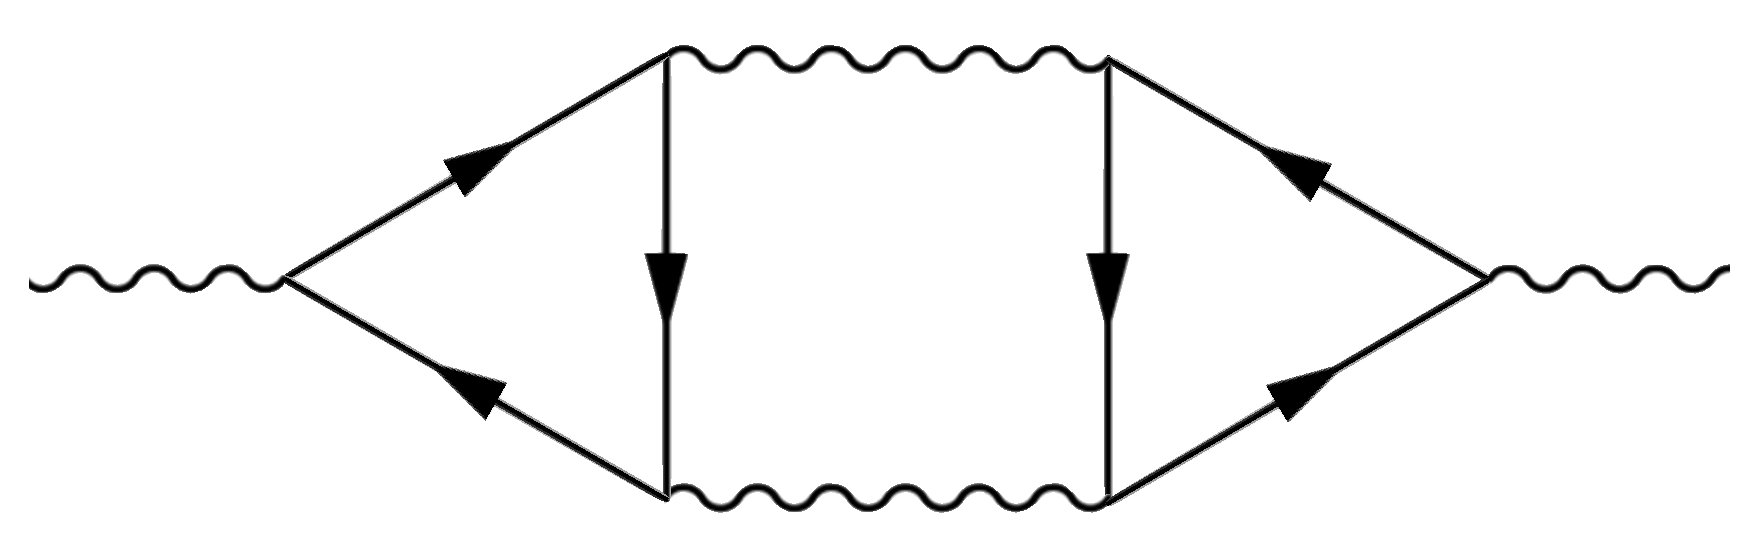
\includegraphics[scale=.25]{imgs/gauge_anomaly}
	\end{center}
\caption{\small ゲージボソンの質量に寄与するFeynman図。} \label{anomalous gauge boson mass}
\end{figure}

自然性の議論を用いれば、ゲージボソン質量の下限まで導くことができる。ツリーレベルでは質量ゼロのゲージボソンから出発し、第$N$クォークが三角形ループ内を伝播する、図\ref{anomalous gauge boson mass}に示したFeynman図を考えよう。アノマリーに詳しい読者なら、このグラフが、カイラルアノマリーの特徴である三角形フェルミオン図二つを、二本の光子線で貼り合わせたものであることに気づくだろう。この3ループ図にはUV発散があるが、ゲージ不変性を保つように正則化する方法はない。この図を低エネルギーEFTでマッチングするには、他の項に加えて、次の質量をもつゲージボソンの質量項を加える必要がある。
%
\begin{align} \label{m_A}
	m_A^2 \sim \left[\frac{1}{(4 \pi)^2}\right]^3 \times (e q_N)^6 \times (2 y v)^2 . 
\end{align}
%
右辺の三つの因子の起源は明らかだろう。各ループに対して一つのループ因子$1/(4 \pi)^2$、各頂点に対して一つの因子$e q_N$があり、ツリーレベルではゲージボソン質量をゼロと仮定したため、フェルミオン質量$2 y v$が、この図に現れる唯一の質量スケールである。また、式\eqref{m_A}は、純粋に低エネルギーEFTの文脈で定義される量を用いて、次のように書き換えられる。
%
\begin{align} \label{m_A 2}
	m_A^2 \sim \left(\frac{e}{4 \pi}\right)^6 \times \left(\sum_{j=1}^{N-1} q_j^3 \right)^2 \times \Lambda^2 ,
\end{align}
% 
ここで$\Lambda$はEFTの強結合スケールである。\emph{後から振り返れば}、実際には次の考察に基づいて、この結果を推測することもできた。
%
\begin{enumerate}
	\item EFTの強結合スケールが、この問題の唯一のスケールである。
	\item Lagrangianは$e \to -e, A_\mu \to - A_\mu$のもとで不変であるため、物理量は$e$の二乗にしか依存しえない。
	\item アノマリー係数は、$U(1)$が実際に対称性であるかどうかを制御する量であるため、質量がこの係数に比例するのは理にかなっている。
	\item Lagrangianは$e \to -e, q_j \to - q_j$のもとで不変であるため、$e$の各因子には$q_j$の因子が伴うはずである。
\end{enumerate}
%
式\eqref{m_A 2}の表式は、実際には非常に一般的であり、自然性に基づいて、アノマリーをもつフェルミオンの組み合わせを含むEFTにおける、Abelianゲージ場の質量の下限を与える。



\subsectionlink{さらに学ぶための文献}

カイラル摂動論に関する、より詳しい総説として、文献~\cite{Ecker:1994gg,Pich:1995bw,Scherer:2002tk}がある。Goldstoneモードの一般的なEFTについては、総説~\cite{Burgess:1998ku,Pich:2018ltt}が重点的に扱っている。アノマリーについては文献~\cite{Harvey:2005it,Bilal:2008qx}、アノマリーをもつYang-Mills理論については文献\cite{Preskill:1990fr}で、さらに詳しく学ぶことができる。




\newpage


